% !TEX program = xelatex
% ============================================================
%  计算机图形学实验报告 —— 实验一：直线的生成
% ============================================================

\documentclass[a4paper,12pt]{ctexart}

% ---------- 页面与页眉 ----------
\usepackage[a4paper,left=2.5cm,right=2.5cm,top=2.5cm,bottom=2.5cm]{geometry}
\usepackage{fancyhdr}
\setlength{\headheight}{14.5pt}
\pagestyle{fancy}
\fancyhf{}
\fancyhead[L]{计算机图形学实验报告}
\fancyhead[R]{\expname}
\fancyfoot[C]{\thepage}
\renewcommand{\headrulewidth}{0.4pt}

% ---------- 通用宏包 ----------
\usepackage{array}
\usepackage{booktabs}
\usepackage{graphicx}
\usepackage{xcolor}
\usepackage{amsmath,amssymb}
\usepackage{caption}
\usepackage{enumitem}
\usepackage{float}

% ---------- 代码环境 ----------
\usepackage{listings}
\definecolor{codegray}{rgb}{0.5,0.5,0.5}
\definecolor{codegreen}{rgb}{0,0.5,0}
\definecolor{codepurple}{rgb}{0.58,0,0.82}
\definecolor{codebg}{rgb}{0.97,0.97,0.97}
\lstset{
    backgroundcolor=\color{codebg},
    basicstyle=\ttfamily\small,
    commentstyle=\color{codegreen}\itshape,
    keywordstyle=\color{blue}\bfseries,
    stringstyle=\color{codepurple},
    numberstyle=\tiny\color{codegray},
    numbers=left,
    numbersep=8pt,
    frame=single,
    rulecolor=\color{black!30},
    breaklines=true,
    breakatwhitespace=true,
    showstringspaces=false,
    tabsize=4,
    captionpos=b,
    xleftmargin=1em,
    xrightmargin=1em,
    columns=flexible
}
\lstdefinestyle{cppstyle}{language=C++}

% ---------- 章节标题外观 ----------
\ctexset{
    section/format = \Large\bfseries\heiti,
    subsection/format = \large\bfseries\heiti
}

% ============================================================
%  实验元信息
% ============================================================
\newcommand{\expname}{实验一\quad 直线的生成}
\newcommand{\expscore}{}
\newcommand{\expdate}{2026 年 5 月 9 日}
\newcommand{\expteacher}{霍鑫}
\newcommand{\expauthor}{张致远}
\newcommand{\expclass}{信计23-1}
\newcommand{\expid}{2023213980}

% ============================================================
\begin{document}

% ---------- 封面表头 ----------
\begin{center}
    {\zihao{2}\heiti 计算机图形学实验报告}
\end{center}
\vspace{0.5em}

\renewcommand{\arraystretch}{1.6}
\noindent
\begin{tabular}{|>{\centering\arraybackslash}m{2.2cm}|m{4.4cm}|>{\centering\arraybackslash}m{2.2cm}|m{4.4cm}|}
    \hline
    \textbf{实验名称} & \multicolumn{3}{l|}{\expname} \\ \hline
    \textbf{评分}     & \expscore   & \textbf{实验日期} & \expdate    \\ \hline
    \textbf{指导教师} & \expteacher & \textbf{姓名}     & \expauthor  \\ \hline
    \textbf{专业班级} & \expclass   & \textbf{学号}     & \expid      \\ \hline
\end{tabular}
\vspace{1.5em}

% ============================================================
%  一、实验目的
% ============================================================
\section{实验目的}

\begin{enumerate}[leftmargin=2em,itemsep=0.2em]
    \item 理解光栅图形系统中直线段扫描转换的基本思想，体会"用离散像素逼近连续直线"这一图形学核心问题。
    \item 掌握 DDA 算法、中点画线算法以及 Bresenham 算法的数学推导与实现细节。
    \item 通过对三种算法的实现与比较，分析它们在效率、误差、可移植性等方面的差异，重点掌握 \textbf{Bresenham 直线生成算法} 的递推逻辑。
    \item 熟悉 OpenGL 编程基本框架，能够利用 \texttt{GL\_POINTS} 模式按算法逐像素绘制图元。
\end{enumerate}

% ============================================================
%  二、实验要求
% ============================================================
\section{实验要求}

\textbf{实验环境：}
\begin{itemize}[leftmargin=2em,itemsep=0.2em]
    \item 实验设备：PC 机一台
    \item 操作系统：Windows 11
    \item 开发工具：Visual Studio 2022 + OpenGL（freeglut 3.4.0）
    \item 编程语言：C++
\end{itemize}

\textbf{实验内容：}
\begin{enumerate}[leftmargin=2em,itemsep=0.2em]
    \item 在屏幕上分别用 DDA 算法、中点画线算法、Bresenham 算法绘制同一条直线段；
    \item 不同算法采用不同颜色或线型加以区别，便于对比生成结果；
    \item 通过键盘交互切换显示某一种或全部算法的输出，便于观察像素分布；
    \item 重点验证 Bresenham 算法在 $0 \le k \le 1$ 第一象限的正确性，并扩展到任意斜率。
\end{enumerate}

% ============================================================
%  三、关键算法及实现原理
% ============================================================
\section{关键算法及实现原理}

设直线段两端点为 $P_1(x_1,y_1)$ 与 $P_2(x_2,y_2)$，记
$\Delta x = x_2-x_1,\;\Delta y = y_2-y_1$，斜率 $k = \Delta y / \Delta x$。
不失一般性，下文以 $0 \le k \le 1$、$x_1 < x_2$ 为典型情况推导。

\subsection{DDA（数字微分分析器）算法}

DDA 利用直线的微分方程
$\dfrac{dy}{dx}=k$，沿 $x$ 方向每步增 $1$，则 $y$ 方向相应增加 $k$：
\[
    x_{i+1}=x_i+1,\qquad y_{i+1}=y_i+k.
\]
绘制时取 $\mathrm{round}(y_{i+1})$ 作为像素纵坐标。算法直观，但需要浮点加法和取整运算，效率较低。

\subsection{中点画线算法}

将直线方程写为 $F(x,y)=ax+by+c=0$，其中 $a=\Delta y,\;b=-\Delta x$。
当像素 $(x_i,y_i)$ 已绘制后，下一像素只可能是 $E(x_i+1,y_i)$ 或 $NE(x_i+1,y_i+1)$。
取两者中点 $M(x_i+1, y_i+\tfrac{1}{2})$，构造判别式
\[
    d_i = F(x_i+1, y_i+\tfrac{1}{2}) = a(x_i+1) + b(y_i+\tfrac{1}{2}) + c .
\]
$d_i<0$ 时中点在直线下方，下一像素取 $NE$；否则取 $E$。利用增量推导得：
\[
    d_{i+1} =
    \begin{cases}
        d_i + a + b, & d_i<0\;(\text{走 } NE) \\
        d_i + a,     & d_i\ge 0\;(\text{走 } E)
    \end{cases}
\]
初值 $d_1 = a + b/2$。为消除小数，可整体乘 $2$，即令 $D = 2d$，全部用整数运算。

\subsection{Bresenham 算法（重点）}

Bresenham 同样采用递推思想，但以"误差量"代替"中点判别式"，物理含义更直观。
设当前像素为 $(x_i,y_i)$，理想直线在 $x_i+1$ 处的纵坐标为 $y_i+k$，
当累计偏离 $\ge 0.5$ 时纵坐标进 $1$。

为避免浮点运算，令
\[
    P_i = 2\Delta x \cdot e_i - \Delta x ,
\]
则判别条件 $e_i \ge 0.5$ 等价于 $P_i \ge 0$。代入递推得：
\[
    P_{i+1} =
    \begin{cases}
        P_i + 2\Delta y - 2\Delta x, & P_i \ge 0 \\
        P_i + 2\Delta y,             & P_i < 0
    \end{cases}
    \qquad
    P_1 = 2\Delta y - \Delta x.
\]

\textbf{算法步骤}（$0\le k\le 1$）：
\begin{enumerate}[leftmargin=2em,itemsep=0.2em]
    \item 画起点 $(x_1,y_1)$，计算误差初值 $P_1 = 2\Delta y - \Delta x$，置 $i=1$；
    \item 求下一像素 $x_{i+1}=x_i+1$；若 $P_i \ge 0$ 则 $y_{i+1}=y_i+1$，否则 $y_{i+1}=y_i$；
    \item 画点 $(x_{i+1}, y_{i+1})$；
    \item 更新误差：$P_i \ge 0$ 时 $P_{i+1}=P_i+2\Delta y-2\Delta x$，否则 $P_{i+1}=P_i+2\Delta y$；
    \item $i=i+1$，若 $i<\Delta x+1$ 转步骤 2，否则结束。
\end{enumerate}

\textbf{对一般斜率的推广：}\ 若 $|k|>1$，则交换 $x,y$ 角色（沿 $y$ 步进）；若 $\Delta x<0$ 或 $\Delta y<0$，
通过 $\mathrm{sign}$ 控制步进方向即可，本质算法保持不变。

\subsection{三种算法对比}

\begin{table}[H]
\centering
\renewcommand{\arraystretch}{1.3}
\begin{tabular}{lccc}
\toprule
对比维度 & DDA & 中点画线 & Bresenham \\
\midrule
基本运算  & 浮点加 + 取整 & 整数加 & 整数加（仅加减）\\
单像素开销 & 较大 & 小 & \textbf{最小} \\
误差分析 & 浮点累计误差 & 几何意义清晰 & 误差离散可控 \\
推广性 & 易扩展到曲线 & 易扩展到圆/椭圆 & 易扩展到圆/椭圆 \\
工程应用 & 教学 / 原型 & 较常用 & \textbf{硬件实现首选} \\
\bottomrule
\end{tabular}
\caption{三种直线生成算法的比较}
\end{table}

% ============================================================
%  四、程序调试中的问题
% ============================================================
\section{程序调试中的问题}

\begin{enumerate}[leftmargin=2em,itemsep=0.4em]
    \item \textbf{斜率范围的限制问题。}\ 最初仅按指导书给定步骤实现 $0\le k\le 1$ 的情况，
        当输入端点斜率为负或大于 $1$ 时输出明显错误。\\
        \textit{解决：}\ 在算法入口对端点进行预处理——根据 $|\Delta x|$ 与 $|\Delta y|$ 的大小决定主步进方向，
        并通过 $\mathrm{sign}(\Delta x)$、$\mathrm{sign}(\Delta y)$ 控制步进方向，使 Bresenham 适用于全部 8 个八分圆。

    \item \textbf{OpenGL 坐标系与窗口像素的映射问题。}\ 默认正交投影中，
        \texttt{glVertex2i} 接收的是世界坐标，与窗口像素并非一一对应。
        若不显式设置投影矩阵，绘制结果会被自动缩放，难以观察单像素差异。\\
        \textit{解决：}\ 调用 \texttt{gluOrtho2D(0, W, 0, H)} 将世界坐标显式设为窗口像素坐标，
        并使用 \texttt{glPointSize(1.0)} 保证一个图元对应一个屏幕像素。

    \item \textbf{DDA 浮点累计误差的可视化。}\ 当直线较长（如跨越窗口）时，
        DDA 与 Bresenham 的输出在末端有 $1\sim 2$ 像素的偏差。\\
        \textit{解决：}\ 这并非 bug，而是浮点误差累积的预期表现。
        通过将 DDA 与 Bresenham 平移 $10$ 像素并行绘制，可直观对比两者末端偏差，
        进一步说明 Bresenham 在长线段上的优越性。

    \item \textbf{端点丢失问题。}\ 初版循环条件写为 \texttt{while(x < x2)}，
        终点像素 $(x_2,y_2)$ 未被绘制。\\
        \textit{解决：}\ 改为 \texttt{for(int i=0; i<=dx; ++i)} 或在循环结束后显式补绘端点。
\end{enumerate}

% ============================================================
%  五、程序运行结果或数据
% ============================================================
\section{程序运行结果或数据}

程序窗口大小 $600\times 600$，分别使用三种算法绘制端点
$P_1(50,80)$、$P_2(550,420)$ 的同一条直线段，并将 DDA、中点、Bresenham 的输出
分别在 $y$ 方向偏移 $-10,0,+10$ 像素以便对比。颜色约定：

\begin{itemize}[leftmargin=2em,itemsep=0.2em]
    \item \textcolor{red}{红色} —— Bresenham 算法
    \item \textcolor{green!60!black}{绿色} —— 中点画线算法
    \item \textcolor{blue}{蓝色} —— DDA 算法
\end{itemize}

\begin{figure}[H]
    \centering
    % 占位：将实际运行截图命名为 exp1_result.png 放入 figures/ 目录后取消下一行注释
    % 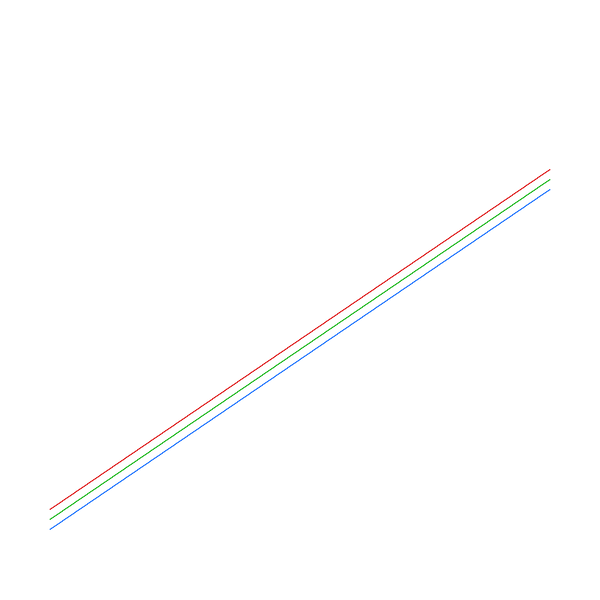
\includegraphics[width=0.7\linewidth]{figures/exp1_result.png}
    \fbox{\parbox[c][6cm][c]{0.7\linewidth}{\centering\itshape
        运行截图占位\\（请将程序运行截图保存为\\
        \texttt{figures/exp1\_result.png} 后取消代码中 \texttt{includegraphics} 的注释）}}
    \caption{三种直线生成算法的对比效果}
\end{figure}

\textbf{观察结论：}
\begin{itemize}[leftmargin=2em,itemsep=0.2em]
    \item 三条直线的整体走向完全一致，验证算法实现正确；
    \item 在斜率较缓（$k\approx 0.68$）的情形下，中点与 Bresenham 输出的像素序列完全相同——
        这是理论上可证明的等价关系；
    \item DDA 在直线两端附近的像素分布与另两者偶有 $1$ 像素差异，符合浮点取整误差的预期。
\end{itemize}

% ============================================================
%  六、实验收获及体会
% ============================================================
\section{实验收获及体会}

通过本次实验，我深入体会到了"光栅化"在计算机图形学中的核心地位——再优雅的几何模型，
最终都要经过扫描转换才能呈现在屏幕上。三种算法的演进过程
（DDA $\to$ 中点 $\to$ Bresenham）也是一次典型的算法优化历程：
\textbf{从浮点到整数、从乘法到加法、从绝对计算到增量递推}，
每一步都体现了"用代数等价变形换取硬件友好性"的工程思想。

特别是 Bresenham 算法，仅用整数加减就能精确逼近真实直线，
这种巧思在嵌入式 GPU、图形硬件流水线中至今仍被广泛采用。
此外，本次实验也让我熟悉了 OpenGL 的基本框架：
显示回调 $\to$ 投影矩阵 $\to$ 图元绘制 $\to$ 缓冲区交换，
为后续圆弧、曲线、填充等实验打下了基础。

% ============================================================
%  七、参考源程序
% ============================================================
\section{参考源程序}

完整 OpenGL/C++ 源程序如下，按 \texttt{1/2/3} 键切换显示算法，按 \texttt{0} 键同时显示三种算法。

\begin{lstlisting}[style=cppstyle,caption={直线生成算法对比 —— 完整源代码}]
// ============================================================
//  实验一：直线的生成 —— DDA / 中点 / Bresenham
//  编译：cl /EHsc exp1.cpp freeglut.lib opengl32.lib glu32.lib
// ============================================================
#include <GL/freeglut.h>
#include <cmath>
#include <cstdio>
#include <algorithm>

const int W = 600, H = 600;
int  mode = 0;          // 0:全部 1:DDA 2:中点 3:Bresenham
int  px1 = 50, py1 = 80, px2 = 550, py2 = 420;

// ---------- 工具：单像素绘制 ----------
inline void putPixel(int x, int y) {
    glBegin(GL_POINTS);
    glVertex2i(x, y);
    glEnd();
}

// ---------- 1. DDA 算法 ----------
void DDA_Line(int x1, int y1, int x2, int y2) {
    int dx = x2 - x1, dy = y2 - y1;
    int steps = std::max(std::abs(dx), std::abs(dy));
    float xInc = (float)dx / steps;
    float yInc = (float)dy / steps;
    float x = (float)x1, y = (float)y1;
    for (int i = 0; i <= steps; ++i) {
        putPixel((int)std::lround(x), (int)std::lround(y));
        x += xInc;  y += yInc;
    }
}

// ---------- 2. 中点画线算法 (0 <= k <= 1) ----------
void Midpoint_Line(int x1, int y1, int x2, int y2) {
    int a = y1 - y2, b = x2 - x1;
    int d  = 2 * a + b;
    int d1 = 2 * a;
    int d2 = 2 * (a + b);
    int x = x1, y = y1;
    putPixel(x, y);
    while (x < x2) {
        if (d < 0) { ++x; ++y; d += d2; }
        else       { ++x;       d += d1; }
        putPixel(x, y);
    }
}

// ---------- 3. Bresenham 算法（任意斜率） ----------
void Bresenham_Line(int x1, int y1, int x2, int y2) {
    int dx = std::abs(x2 - x1), dy = std::abs(y2 - y1);
    int sx = (x1 < x2) ? 1 : -1;
    int sy = (y1 < y2) ? 1 : -1;
    int err = dx - dy;
    int x = x1, y = y1;
    while (true) {
        putPixel(x, y);
        if (x == x2 && y == y2) break;
        int e2 = 2 * err;
        if (e2 > -dy) { err -= dy; x += sx; }
        if (e2 <  dx) { err += dx; y += sy; }
    }
}

// ---------- 显示回调 ----------
void display() {
    glClear(GL_COLOR_BUFFER_BIT);
    glPointSize(1.0f);

    // 蓝色：DDA   ( y - 10 )
    if (mode == 0 || mode == 1) {
        glColor3f(0.0f, 0.4f, 1.0f);
        DDA_Line(px1, py1 - 10, px2, py2 - 10);
    }
    // 绿色：中点   ( 原位 )
    if (mode == 0 || mode == 2) {
        glColor3f(0.0f, 0.7f, 0.0f);
        Midpoint_Line(px1, py1, px2, py2);
    }
    // 红色：Bresenham ( y + 10 )
    if (mode == 0 || mode == 3) {
        glColor3f(1.0f, 0.0f, 0.0f);
        Bresenham_Line(px1, py1 + 10, px2, py2 + 10);
    }
    glFlush();
}

// ---------- 键盘回调 ----------
void keyboard(unsigned char key, int, int) {
    if (key >= '0' && key <= '3') {
        mode = key - '0';
        glutPostRedisplay();
    }
    if (key == 27) std::exit(0);   // ESC 退出
}

// ---------- 初始化 ----------
void init() {
    glClearColor(1.0f, 1.0f, 1.0f, 1.0f);
    glColor3f(0.0f, 0.0f, 0.0f);
    glMatrixMode(GL_PROJECTION);
    gluOrtho2D(0.0, (GLdouble)W, 0.0, (GLdouble)H);
}

int main(int argc, char** argv) {
    glutInit(&argc, argv);
    glutInitDisplayMode(GLUT_SINGLE | GLUT_RGB);
    glutInitWindowSize(W, H);
    glutInitWindowPosition(100, 100);
    glutCreateWindow("Exp.1  Line Generation: DDA / Midpoint / Bresenham");
    init();
    glutDisplayFunc(display);
    glutKeyboardFunc(keyboard);
    glutMainLoop();
    return 0;
}
\end{lstlisting}

\end{document}
